% Latex header for doxygen 1.8.6
\documentclass[twoside,12pt]{book}

% Packages required by doxygen
%\usepackage{alltt}
%\usepackage{array}
\usepackage{doxygen}
\usepackage{graphicx}
\usepackage{calc}
\usepackage{float}
\usepackage{ifthen}
\usepackage{tabularx}
\usepackage{multirow}
\usepackage{multicol}
\usepackage{makeidx}
\usepackage{textcomp}
\usepackage{colortbl}
\usepackage[table]{xcolor}
\usepackage{longtable,booktabs}
\usepackage{tabu}

% Font selection
\usepackage[utf8]{inputenc}
%\usepackage[T1]{fontenc}
\usepackage{mathptmx}
\usepackage[scaled=.90]{helvet}
\usepackage{courier}
\usepackage{amssymb}
\usepackage{upgreek}
\usepackage{amsfonts}
\usepackage{mathrsfs}
\usepackage{algorithm}
\usepackage{algorithmicx}
\usepackage{sectsty}
\renewcommand{\familydefault}{\sfdefault}
\allsectionsfont{%
  \fontseries{bc}\selectfont%
  \color{darkgray}%
}
\renewcommand{\DoxyLabelFont}{%
  \fontseries{bc}\selectfont%
  \color{darkgray}%
}

% Page & text layout
\usepackage{geometry}
\geometry{%
  a4paper,%
  top=2.5cm,%
  bottom=2.5cm,%
  left=2.5cm,%
  right=2.5cm%
}
\tolerance=750
\hfuzz=15pt
\hbadness=750
\setlength{\emergencystretch}{15pt}
\setlength{\parindent}{0cm}
\setlength{\parskip}{0.2cm}
\makeatletter
\renewcommand{\paragraph}{%
  \@startsection{paragraph}{4}{0ex}{-1.0ex}{1.0ex}{%
    \normalfont\normalsize\bfseries\SS@parafont%
  }%
}
\renewcommand{\subparagraph}{%
  \@startsection{subparagraph}{5}{0ex}{-1.0ex}{1.0ex}{%
    \normalfont\normalsize\bfseries\SS@subparafont%
  }%
}
\makeatother

% Headers & footers
\usepackage{fancyhdr}
\pagestyle{fancy}
\fancyhead[LE]{\fancyplain{}{\bfseries\thepage}}
\fancyhead[CE]{\fancyplain{}{}}
\fancyhead[RE]{\fancyplain{}{\bfseries\leftmark}}
\fancyhead[LO]{\fancyplain{}{\bfseries\rightmark}}
\fancyhead[CO]{\fancyplain{}{}}
\fancyhead[RO]{\fancyplain{}{\bfseries\thepage}}
\fancyfoot[LE]{\fancyplain{}{}}
\fancyfoot[CE]{\fancyplain{}{}}
\fancyfoot[RE]{\fancyplain{}{\bfseries\scriptsize Generated on Thu Feb 22 2018 13\-:42\-:02 for My Project by Doxygen }}
\fancyfoot[LO]{\fancyplain{}{\bfseries\scriptsize Generated on Thu Feb 22 2018 13\-:42\-:02 for My Project by Doxygen }}
\fancyfoot[CO]{\fancyplain{}{}}
\fancyfoot[RO]{\fancyplain{}{}}
\renewcommand{\footrulewidth}{0.4pt}
\renewcommand{\chaptermark}[1]{%
  \markboth{#1}{}%
}
\renewcommand{\sectionmark}[1]{%
  \markright{\thesection\ #1}%
}

\usepackage[Sonny]{fncychap}

% Indices & bibliography
\usepackage{natbib}
\usepackage[titles]{tocloft}
\setcounter{tocdepth}{2}
\setcounter{secnumdepth}{2}
\makeindex

% Hyperlinks (required, but should be loaded last)
\usepackage{ifpdf}
\ifpdf
  \usepackage[pdftex,pagebackref=true]{hyperref}
\else
  \usepackage[ps2pdf,pagebackref=true]{hyperref}
\fi
\hypersetup{%
  colorlinks=true,%
  linkcolor=blue,%
  citecolor=blue,%
  unicode%
}

% Custom commands
\newcommand{\clearemptydoublepage}{%
  \newpage{\pagestyle{empty}\cleardoublepage}%
}

\usepackage{amsmath}

% In case of problems with tex compilation
\newcommand{\+}{}

\newlength{\drop}

%===== C O N T E N T S =====

\begin{document}

% Titlepage & ToC
\hypersetup{pageanchor=false}
\pagenumbering{roman}
\begin{titlepage}
    \drop=0.1\textheight
    \centering
    \vspace*{\baselineskip}
    \rule{\textwidth}{1.6pt}\vspace*{-\baselineskip}\vspace*{2pt}
    \rule{\textwidth}{0.4pt}\\[\baselineskip]
    {\LARGE EOPDev \\[0.3\baselineskip] Version 1.0.0}\\[0.2\baselineskip]
    \rule{\textwidth}{0.4pt}\vspace*{-\baselineskip}\vspace{3.2pt}
    \rule{\textwidth}{1.6pt}\\[\baselineskip]
    \scshape
    Elimination of Electron Repulsion Integrals\\
    from Fragment-Based Methods of Quantum Chemistry\\
    \vspace{2.0pt}
    A Plugin to Psi4\par
    \vspace*{2\baselineskip}
    By \\[\baselineskip]
    {\Large Bartosz Błasiak \par}
    {\itshape Wrocław University of Science and Technology\par}
    \vfill
    \vspace*{2\baselineskip}
    Funded by \\[\baselineskip]
    {\Large National Science Centre, Kraków, Poland\par}
    {\itshape Grant No. 2016/23/P/ST4/01720\par}
    {\Large H2020 Marie Skłodowska-Curie Actions Co-Fund (POLONEZ)\par}
    {\itshape Grant No. 665778\par}
        \begin{center}
            
\includegraphics[width=0.1\linewidth]{eu.pdf}
        \end{center}
    \vfill
    {\scshape November 2020} \\
    {\large License: LGPL-2.1}\par
%\vspace*{7cm}
%\begin{center}%
%{\Large EOPDev 1.0.0}\\
%\vspace*{1cm}
%{\large }Elimination of Electron Repulsion Integrals\\from Fragment-Based Methods of Quantum Chemistry\\
%\vspace*{1cm}
%{\small Generated by Doxygen 1.8.6}\\
%\vspace*{0.5cm}
%{\small Tue Nov 17 2020 11:26:02}\\
%\end{center}
\end{titlepage}
\clearemptydoublepage
\tableofcontents
\clearemptydoublepage
\begin{figure}[t]
\centering
%\colorbox{background-color}{
\fbox{
\begin{minipage}{1.0\textwidth}
\hfill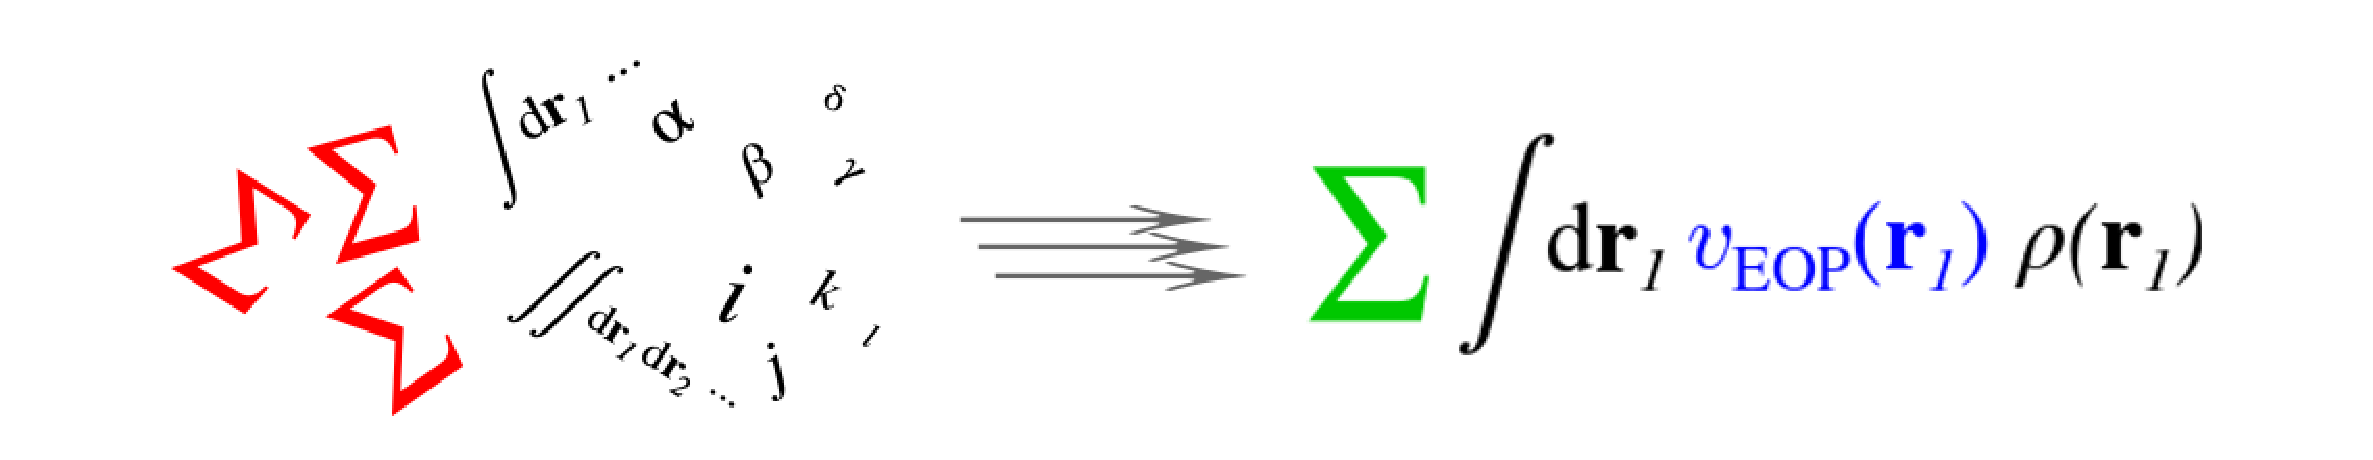
\includegraphics[height=30mm]{toc.eps}\hspace*{\fill}
\\
Effective one-electron operators can be systematically used to convert fragment-based methods
into effective fragment potentials.
\end{minipage}
} %}
\end{figure}
\clearemptydoublepage
\pagenumbering{arabic}
\hypersetup{pageanchor=true}

%--- Begin generated contents ---
